\section{Ausgangslage}
\label{sec:Ausgangslage}

\begin{wrapfigure}{l}{0.55\textwidth}
  \begin{center}
    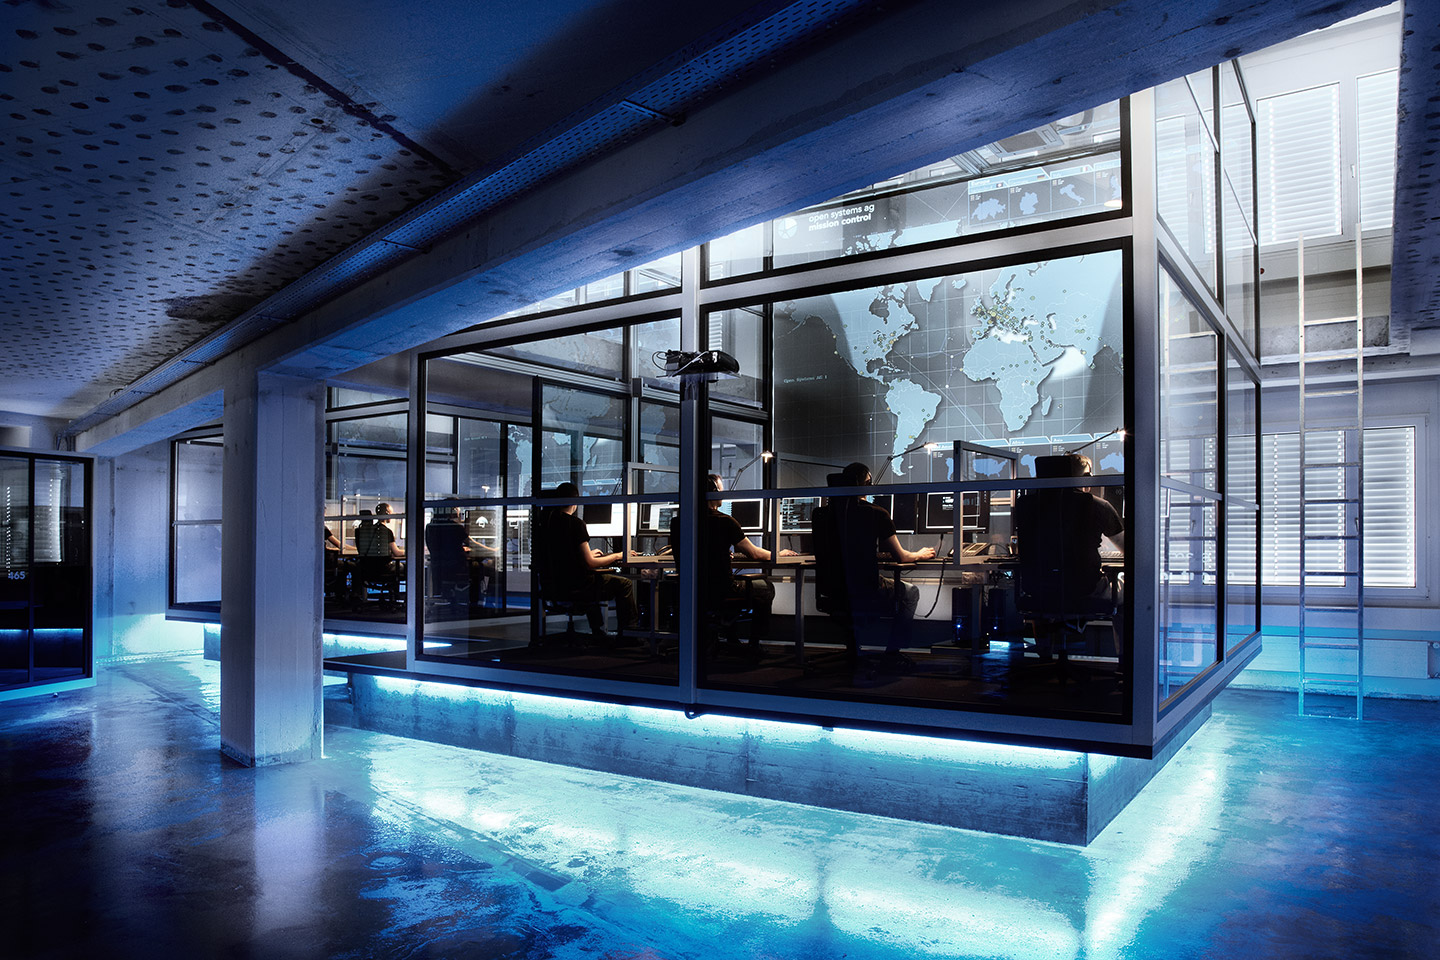
\includegraphics[clip,scale=0.15]{mainpart/anforderungen/img/gallery_mc_01}
    \caption{Mission Control Center}
  \end{center}
\end{wrapfigure}


Die Firma \osag{} betreibt ein weltweites Netz von \acs{IPsec} \acs{VPN} Verbindungen. Die Kunden der \osag kommen unter anderem aus den Branchen: Finanzen, Versicherungen, Regierung, Detail Handel und weiteren. Daher ist es für \osag sehr wichtig, dass die Verbindungen konstant überwacht werden. Zu diesem Zweck betreibt die \osag auch zwei Mission Control Center\footnotemark[1] mit den Standorten Zürich und Sydney. So ist ein \enquote{Follow-the-Sun} 24/7 Betrieb möglich.

\footnotetext[1]{Bild: \url{http://open.ch}}

Die Aufgabe dieser Mission Control Center ist es die \acs{VPN}-Verbindungen konstant zu überwachen und auf Kunden Probleme zu reagieren. Anders als bei Firmen mit typischem First-, Second- und Third-Level Support sind die Mission Control Center stets von Ingenieuren besetzt, die sich Kundenproblem so direkt annehmen können und auch komplexe Probleme in kürzester Zeit lösen. Probleme, die vermehrt auftreten werden, dort auch gleich mit einer automatisierten Lösung versehen, sodass sie beim erneuten Auftreten nicht durch einen Menschen bearbeitet werden müssen.

Im Sinne dieser Automatisierungs-Bestrebung soll mit dieser Arbeit auch das Detektieren von Paket-Verlusten und die Bestimmung der MTU gelöst werden.
Das manuelle Überprüfen von Paket-Verlusten und bestimmen von Fragmentierungsproblem nimmt viel Zeit in Anspruch. Es soll nun eine Applikation programmiert werden, womit sich diese Arbeit automatisieren lässt, sodass mit weniger Aufwand eine bessere Verbindungsqualität gewährleistet werden kann.


\subsection{Produktfunktion}
Es soll eine Applikation (\tool{}) entwickelt werden die das Erkennen und Diagnostizieren von Problemen bei \acs{IPsec} \acs{VPN}-Verbindungen vereinfacht. Dabei soll das Tool die Möglichkeit bieten passiv Paket-Verluste zu erkennen sowie aktiv die \acs{MTU} zu bestimmen. Die Applikation wird als konstant laufender Service konzipiert und bietet daher keine grafische Oberfläche, sondern nur ein Commandline-Interface. Für die Kommunikation mit den Benutzern sollen Log-Einträge verwendet werden.

\subsection{Benutzercharakteristik}
Die Benutzer der Applikation sind Netzwerkadministratoren \& Informatik-Ingenieure die \acs{IPsec} \acs{VPN} Tunnels betreiben. Ein grosses Mass an technischem Verständnis und Erfahrung im Zusammenhang mit \acs{IPsec} und \acs{VPN}-Verbindungen kann deshalb vorausgesetzt werden. Sie haben auch ausgeprägte Kenntnisse von der Bedienung von Linux und Kommandozeilen Applikationen.

\subsection{Abhängigkeiten}
Das Tool wird als eigenständige Applikation entwickelt und kann zur Fehlerdiagnose bei beliebigen \acs{IPsec} Tunnels eingesetzt werden. Es gibt keine enge Bindung zu externen Applikationen oder zur Infrastruktur der \osag{}.